\documentclass{bschlangaul-aufgabe}
\bLadePakete{java}
\usepackage{tikz}
\begin{document}
\bAufgabenMetadaten{
  Titel = {Das Haus des Nikolaus},
  Thematik = {Nikolaus},
  Referenz = AUD.Algorithmenmuster.Backtracking.Nikolaus,
  RelativerPfad = Module/30_AUD/60_Algorithmenmuster/50_Backtracking/Aufgabe_Nikolaus.tex,
  ZitatSchluessel = aud:ab:3,
  ZitatBeschreibung = {Diese Aufgabe stammt von der Website oberstufeninformatik.de. Die
Materialien sind nicht Freeware, sondern Beerware. Voraussetzung für
den Einsatz ist, dass der Benutzer ein Bier zum Wohle des Autors Horst
Gierhardt trinkt, Seite 2-3, Aufgabe 3},
  BearbeitungsStand = mit Lösung,
  Korrektheit = unbekannt,
  Ueberprueft = {unbekannt},
  Stichwoerter = {Backtracking},
}

\noindent
Hier ist das \emph{„Haus des Nikolaus“} mit einer bestimmten
Nummerierung der Eckpunkte vorgegeben. Es sollen alle Lösungen zum
Zeichnen der Figur in einem Zug gefunden werden. Eine Lösung könnte dann
in der Form 123451352 ausgegeben werden. Das Programm soll eine einfache
Anpassung an andere Graphen ermöglichen. Der Ausschluss von gespiegelten
Lösungen ist nicht gefordert.\index{Backtracking}
\footcite[Diese Aufgabe stammt von der Website oberstufeninformatik.de. Die
Materialien sind nicht Freeware, sondern Beerware. Voraussetzung für
den Einsatz ist, dass der Benutzer ein Bier zum Wohle des Autors Horst
Gierhardt trinkt, Seite 2-3, Aufgabe 3]{aud:ab:3}

\begin{center}
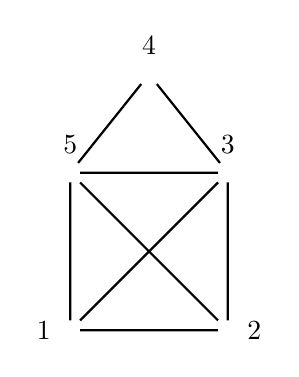
\begin{tikzpicture}[rounded corners=8pt]
\node[label=180:1] (eins) at (0,0) {};
\node[label=0:2] (zwei) at (2,0) {};
\node[label=3] (drei) at (2,2) {};
\node[label=4] (vier) at (1,3.25) {};
\node[label=5] (fünf) at (0,2) {};

\draw[thick]
(eins) -- (fünf) -- (vier) -- (drei) -- (zwei) -- (fünf) -- (drei) -- (eins) -- (zwei);
\end{tikzpicture}
\end{center}

\begin{bExkurs}[Backtracking]
Eine Lösung lässt sich nach dem Prinzip \emph{Versuch und Testen}
ermitteln. Eine vermutete Teillösung muss wieder verworfen werden, wenn
ein Test ihre Ungültigkeit nachgewiesen hat. Man nennt diesen Ansatz
deshalb auch \emph{Rückverfolgen} oder \emph{Backtracking}. Mit diesem
Ansatz lassen sich eine ganze Reihe von Problemen in der Informatik sehr
elegant formulieren und lösen. Hier eine kleine Auswahl (Genaueres dazu
später):

\begin{description}
\item[Acht-Damen-Problem:] Acht Damen sollen so auf ein Schachbrett
gestellt werden, dass keine Dame eine andere bedroht.

\item[Vier-Farben-Problem:] Eine Landkarte soll mit vier Farben so
gefärbt werden, dass benachbarte Länder immer unterschiedliche Farben
bekommen.

\item[Labyrinth-Problem:] Ein Labyrinth mit Sackgassen und Verzweigungen
ist zu durchlaufen, um den Ausgang zu finden.
\end{description}
\end{bExkurs}

\noindent
Konkreter:

\begin{enumerate}
\item Man versucht, eine Kante (Verbindungsstrecke) zu zeichnen, wenn
sie zulässig ist oder noch nicht gezeichnet wurde.

\item Ist das nicht möglich, muss die zuletzt gezeichnete Kante gelöscht
werden.

\item  Ist es möglich, dann hat man das Problem um eine Stufe
vereinfacht.

\item  Hat man durch dieses Verfahren insgesamt 8 Kanten zeichnen
können, hat man eine Lösung gefunden. Jetzt löscht man wieder die
zuletzt gezeichnete Kante und sucht nach weiteren Lösungen.
\end{enumerate}

\subsection{Realisierung des Programms}

\subsubsection{Datenstrukturen}

Die folgende Tabelle gibt an, welche Verbindungslinien zulässig sind
(durch X markiert). Die erste Zeile bedeutet also, dass von Punkt 1 zu
den Punkten 2, 3 und 5 Strecken gezeichnet werden dürfen. Eine solche
Tabelle heißt auch Adjazenzmatrix (von adjazieren; lat.: anwohnen,
anliegen). Eine solche Tabelle lässt sich durch \bJavaCode{boolean[][]
kanteZulaessig}; in einem zweidimensionalen Feld speichern. Eine
entsprechende Tabelle \bJavaCode{boolean[][] kanteGezeichnet;} erfasst dann die
schon gezeichneten Kanten. In einem weiteren eindimensionalen Feld
wird jeweils eine Lösung erfasst.

\subsubsection{Methoden}

Es bieten sich folgende Methoden zur Strukturierung des Programmes an:

\begin{enumerate}
\item \bJavaCode{void initialsiereFelder()}
\item \bJavaCode{void zeichneKante(int von, int nach)}
\item \bJavaCode{void löscheKante(int von, int nach)}
\item \bJavaCode{void gibLösungAus()}
\item \bJavaCode{void versucheKanteZuZeichnen(int start)}: Die rekursive
Methode soll vom Punkt start weitere Kanten zeichen.

\item Das Hauptprogramm:

\begin{minted}{java}
public static void main(String[] arg) {
  initialsiereFelder();
  for (int punktNr = 1; punktNr <= maxPunktAnzahl; punktNr++) {
    lösungsWeg[0] = punktNr; // Startpunkt eintragen
    versucheKanteZuZeichnen(punktNr);
  }
  System.out.println();
  System.out.println("Es ergaben sich " + lösungsAnzahl + " Loesungen.");
}
\end{minted}

\end{enumerate}

\bJavaDatei[firstline=3]{aufgaben/aud/muster/backtracking/Nikolaus}

\end{document}
